\section{Linial's Algorithm}

A useful procedure is one that merges two linearly ordered sets without
discarding the information existing between elements of these two sets. In
\citet*{cardinal:2013} an implementation of such a procedure is defined. Their
implementation allows one to concentrate the computational complexity of this
procedure in the preprocessing phase of their other algorithms. In this chapter
we will detail another possible implementation of such a procedure that is due
to \citet*{linial:1984}. Unfortunately, in this implementation the
computational complexity cannot be split into a preprocessing phase and a query
phase. Nevertheless it is still interesting to understand the ideas behind it.

This procedure solves the problem of Merging under Partial Information, or
\concept{MUPI}. We give a formal definition of this problem,

\begin{problem}
Given a poset \(\P\) that can be covered by two chains \(\A\) and \(\B\), find a
linear extension of \(\P\).
\end{problem}

\begin{figure}
\centering
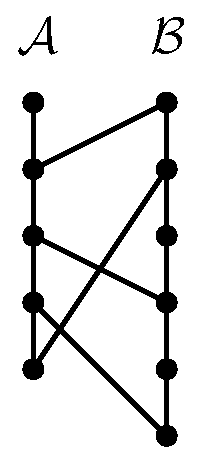
\includegraphics[height=0.2\textheight]{fig/supi/mupi}
\caption{A poset \(\P\) covered by two chains \(\A\) and \(\B\),
input of the MUPI problem.}
\label{fig:supi:mupi}
\end{figure}

\citet*{linial:1984} first proves that the \onethirdtwothird conjecture holds
for width-\(2\) posets, \ie posets that can be covered by two chains. Since one
can always find a good query that when answered will invalidate at
least one third of the possible linear extensions of \(\P\), it is possible to design a
\BigO{\log e(\P)} algorithm that solves the MUPI problem.

\begin{theorem}
Given a poset \(\P\) covered by two chains \(\A\) and \(\B\), we can always find
a query \(x \ask{\le} y\) with \(x \in \A, y \in \B\) such that the probability
that \(x \le y\) lies in the interval \([\sfrac{1}{3}, \sfrac{2}{3}]\).
\end{theorem}

Moreover, in his proof, \citet*{linial:1984} shows that if we consider that \(
a_1\) and \(b_1\) are incomparable and \(\frac{e(\P(a_1 < b_1)}{e(\P)} <
\sfrac{1}{3}\) then there must exist a \(r\) for which either

\begin{displaymath}
\sfrac{1}{3} \le \frac{e(\P(a_1 < b_{r-1})}{e(\P)} \le \sfrac{1}{2}
\end{displaymath}
or
\begin{displaymath}
\sfrac{1}{2} \le \frac{e(\P(a_1 < b_{r})}{e(\P)} \le \sfrac{2}{3}.
\end{displaymath}

All of this is without loss of generality. If \(a_1\) and \(b_1\) are
comparable then either \(a_1\) or \(b_1\) is the minimal element of \(\P\) and
all of its extensions. Hence this minimal element can be removed. We can do so
until \(a_1\) and \(b_1\) are incomparable. If \(\frac{e(\P(a_1 < b_1)}{e(\P)} >
\sfrac{2}{3}\) we can simply revert the roles of \(\A\) and \(\B\) and if
\(\sfrac{1}{3} \le \frac{e(\P(a_1 < b_1)}{e(\P)} \le \sfrac{2}{3}\) then we
simply do not have to do any further research. Also, one can build the same
proof using \(a_m\) and \(b_n\) instead of \(a_1\) and \(b_1\).

\citet*{linial:1984} proposes the following polynomial-time algorithm. We
compute the number of linear extensions of the width-\(2\) poset \(\P\) using
the determinant counting formula. We do so also for every query we could use to
retrieve more information on the total order \(\le\). We then use those counts
to find a pair \((x,y)\) that satisfies \(\sfrac{1}{3} \le \frac{e(\P(x \le
y))}{e(\P)} \le \sfrac{2}{3}\), where \(\P(x \le y)\) denotes the poset obtained
from \(\P\) after adding the constraint that \(x \le y\). Once this pair is
identified, we can effectively make the query and update poset \(\P\) with the
actual answer. We can then recurse on the newly obtained poset. Because of the
successive uses of good queries, the recursion depth, and thus the number of
queries made, is \BigO{\log e(\P)}.

The proof for the determinant counting formula \citet*{linial:1984} uses can be
found in \citet*{mohanty:1979}, we give hereunder the statement of this formula
in the context of Merging under Partial Information.

\begin{theorem}
Let \(\P = \A \cup \B\), where \(\A = (\chain{a_1}{a_m})\) and \(\B =
(\chain{b_1}{b_n})\), and assume \(m \ge n\) without loss of generality. Define
the integers \(\alpha_1,\ldots,\alpha_m,\beta_1,\ldots,\beta_m\) as follows,
\(\beta_i = min\{t \st b_t > a_i\}, \alpha_j = max\{t \st b_t < a_j\}\) and
where the minimum and maximum of an empty set are taken to be \(n + 1\) and
\(0\) respectively. Let \(\binom{n}{k}_{+}\) be defined as

\begin{displaymath}
\binom{n}{k}_{+} =
\begin{dcases*}
0            & if  \(n < 0\)  or \(k < 0\)  or \(k > n\)\\
1            & if \(k = 0\)  or \(k = n\)\\
\binom{n}{k} & otherwise\\
\end{dcases*}.
\end{displaymath}

Then, the number of extensions of \(\P\) is given by

\begin{displaymath}
e(\P) =
\begin{vmatrix}
\binom{\beta_i - \alpha_j}{j - i - 1}_{+}
\end{vmatrix}_{1 \le i , j \le m},
\end{displaymath}

the determinant of a \(m \times m\) matrix.
\end{theorem}

\citet*{mohanty:1979} gives this formula in the context of counting lattice
paths. Let us explain. We want to count the number of paths that go from
\((0,0)\) to \((m,n)\) in a \((m+1) \times (n+1)\) grid. Such a path is a
sequence of \(m+n+1\) integer positions \(( (i_{0},j_{0}) , (i_{1},j_{1}) ,
\ldots , (i_{m+n},j_{m+n}) )\) such that \(i_{k} \ge i_{k-1}\), \(j_{k} \ge
j_{k-1}\) and \(i_{k} + j_{k} = i_{k-1} + j_{k-1} + 1\) for all \(1 \le k \le m
+ n\).  Obviously \((i_{0},j_{0}) = (0,0)\) and \((i_{m+n},j_{m+n}) = (m,n)\).
With these constraints alone we obtain a count of \(\binom{m+n}{n} =
\binom{m+n}{m} \) different paths\footnote{Note that if \(m = n\) and if we add
the condition that \(i_{k} \le j_{k} \Forall 1 \le k \le m + n\) then the path
count corresponds to the \(\nth{n}\) Catalan number \(C_n\).}.
\citet*{mohanty:1979} adds the constraint that \(\alpha_i \le j < \beta_i\) for
all path positions \((i,j)\) with \(i \neq 0\), where \(0 \le
\alpha_1 \le \ldots \le \alpha_m \le n + 1\), \(0 \le \beta_1 \le \ldots \le
\beta_m \le n + 1\) and \(\alpha_i < \beta_i \Forall 1 \le i \le m\) and finds
this determinant counting formula as an answer. The reason the cases \(i = 0\)
can be ignored is because the above constraints suffice to fix
the possible values that \(j\) can take when \(i = 0\).

This problem of counting paths is equivalent to counting the number of possible
outcomes of a merging algorithm on input \((\S_1,\S_2)\), \(\card{\S_1} = m,
\card{\S_2} = n\), provided we know the insertion position \(j\) of the
\(\nth{i}\) element of \(\S_1\) into \(\S_2\) is bounded by \(\alpha_i \le j <
\beta_i\).

We now make a few observations to show that Linial's algorithm runs in
polynomial time:

\begin{enumerate}
\item The values \(\beta_i - \alpha_j\) and \(j - i + 1\) are bounded
linearly in the size of the input. Hence, their size is bounded
logarithmically in the size of the input;
\item The size of the value of the binomial coefficient \(\binom{n}{k}\) is
bounded by a polynomial in \(k\) and \(n\);
\item Using Bareiss algorithm \cite{bareiss:1968}, the computation of a
determinant can be made in polynomial time. Moreover, the size of all computed
values is bounded by some polynomial in the size of the matrix and in the starting
size of the values;
\item For each step there is a polynomial number of possible queries to look for;
\item There are \BigO{\log e(\P)} steps and \(\log e(\P)\) is \BigO{n \log n}.
\end{enumerate}

However, as an anonymous referee pointed out in the peer review of
\citet*{cardinal:2013}, there exists a faster way that does not require computing
all those determinants. We now expose a recurrence relation that can be used
to compute \(e(\P)\) with dynamic programming.

We look at \(a_m\) and \(b_n\). There are three ways \(a_m\) and \(b_n\) can be
related in the partial order we receive as input. Either we know \(a_m < b_n\)
or \(a_m > b_n\), or \(a_m\) and \(b_n\) are incomparable in this partial
order. In the first two cases, we know that one of \(a_m,b_n\) must be the last
element of the set \(\A \cup \B\) when totally ordered. In these cases, \(e(\P) =
e(\P \setminus b_n)\) or \(e(\P) = e(\P \setminus a_m)\) for \(a_m < b_n\) or
\(a_m > b_n\) respectively. Now, if \(a_m\) and \(b_n\) are incomparable in
\(\P\), in the totally ordered set we are building one of \(a_m < b_n\) or \(a_m
> b_n\) will hold true. Hence \(e(\P) = e(\P \setminus b_n) + e(\P \setminus
a_m)\) in this case, since both outcomes for \(a \ask{<} b\) are possible.
Lastly, if \(\card{\A} = 0\) or \(\card{\B} = 0\) then \(e(\P) = 1\). We can thus
express \(e(\P)\) using the following recurrence relation

\begin{displaymath}
e(\P) =
\begin{dcases*}
1            & if \(\card{\A} = 0\) or \(\card{\B} = 0\)\\
e(\P \setminus b_n) & if \(a_m < b_n\)\\
e(\P \setminus a_m) & if \(a_m > b_n\)\\
e(\P \setminus b_n) + e(\P \setminus a_m) & if \(a_m\) and \(b_n\) are
incomparable.\\
\end{dcases*}
\end{displaymath}

Note that if one computes \(e(\P)\) using this recurrence in a dynamic program,
he will also get all values of \(e(\P(a_m < b_s))\) and \(e(\P(a_s < b_n))\) for
free. This is because there is only one possible way tail elements can be
arranged to have \(e(\P(a_m < b_s))\), \ie \(a_m < b_s < b_{s+1} < \ldots <
b_n\). Note that other values \(e(\P(a_i < b_j)\) for any pair \((a_i,b_j)\)
would be trickier to compute. The value of \(e(\P)\) and the number of linear
extensions of all poset extensions \(\P(a_m < b_s)\) and \(\P(a_s < b_n)\) can
thus be computed in \BigO{mn \log e(\P)} time using dynamic programming with a
\(m \times n\) memory tableau containing numbers with values up to \(\log
e(\P)\). Note that posets that are incompatible with the original poset \(\P\),
will be assigned a value \(e = 0\).

Moreover, one can reuse the information obtained via the dynamic program. We
explain how. Suppose we have computed \(e(\P)\) and all \(e(\P(a_m < b_s))\) and
\(e(\P(a_s < b_n))\) using the dynamic program. According to these values and
thanks to Linial's proof, we find a good query \(a_m \ask{<} b_s\) to perform.
Depending on the outcome of this query we update the output of the dynamic
program. If \(a_m < b_s\) then we do not have to update anything,
\(\chain{b_s}{b_n}\) can now simply be ignored. Otherwise, \(a_m > b_s\) and
unless \(s = n\) we have to update at most \(s\) cells of the dynamic program
tableau. If the memory tableau of the dynamic program is a \(m \times n\)
tableau \(e = \enum{e_{i,j} = e(\chain{a_1}{a_i} \cup \chain{b_1}{b_j})}\), the
cells to update are \(e_{m,t}\) through \(e_{m,s}\) where \(t \le s\) is \( t =
\min \enum{t \st a_m \text{ and } b_t \text{ are incomparable} }\).

As a final remark, know that it is possible to reduce the computational
complexity of both the construction and the update of the dynamic program. If
we limit ourselves to store \emph{limited precision integers} and perform
\emph{limited precision arithmetic} when adding those integers, then we can
shave off the \(\log e(\P)\) factor in both cases. Hence, if we divide the
execution of the algorithm into a preprocessing phase and a processing phase,
the complexity of the preprocessing phase is \BigO{mn} while doing no
comparisons, and the complexity of the processing phase is \BigO{N \log e(\P)}
using \BigO{\log e(\P)} comparisons where \(N = \max \enum{m,n}\).
